Preferably \emph{bootstrapping} should be done over multiple steps, and that is what
these methods allow us to do.
The idea of $n$-step methods is usually used as an introduction to the algorithmic
idea of \emph{eligibility traces} (Chapter 12), which enable bootstrapping over
multiple time intervals simultaneously.

\section{$n$-step TD Prediction}
\label{sec:n_step_td_prediction}
\begin{figure}[h]
    \centering
    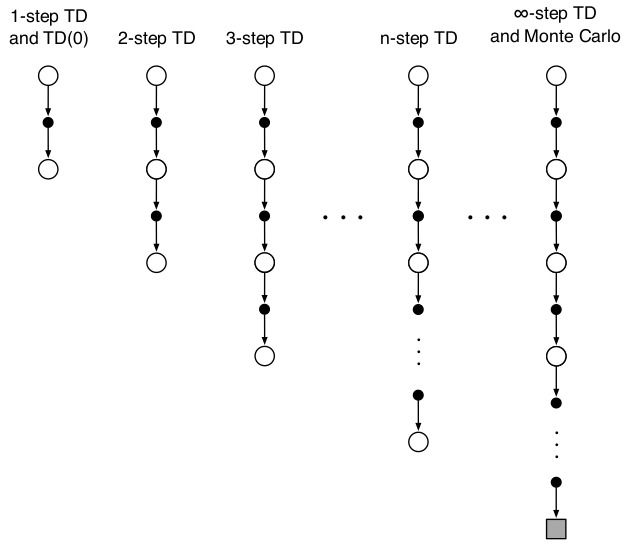
\includegraphics[width=0.7\textwidth]{img/n_step_td.png}
    \caption{The backup diagrams of $n$-step methods.
        These methods form a spectrum ranging from one-step TD methods to Monte
        Carlo methods.}
    \label{fig:7.1}
\end{figure}
\begin{myequation}{7.1}
    G_{t:t+n}\doteq
        R_{t+1}+\gamma R_{t+2}+\cdots+\gamma^{n-1}R_{t+n}+\gamma^nV_{t+n+1}(S_{t+n})
\end{myequation}
\begin{myequation}{7.2}
    V_{t+n}(S_t)\doteq V_{t+n-1}+\alpha\left(G_{t:t+n}-V_{t+n-1}(S_t)\right)
\end{myequation}

\begin{center}
    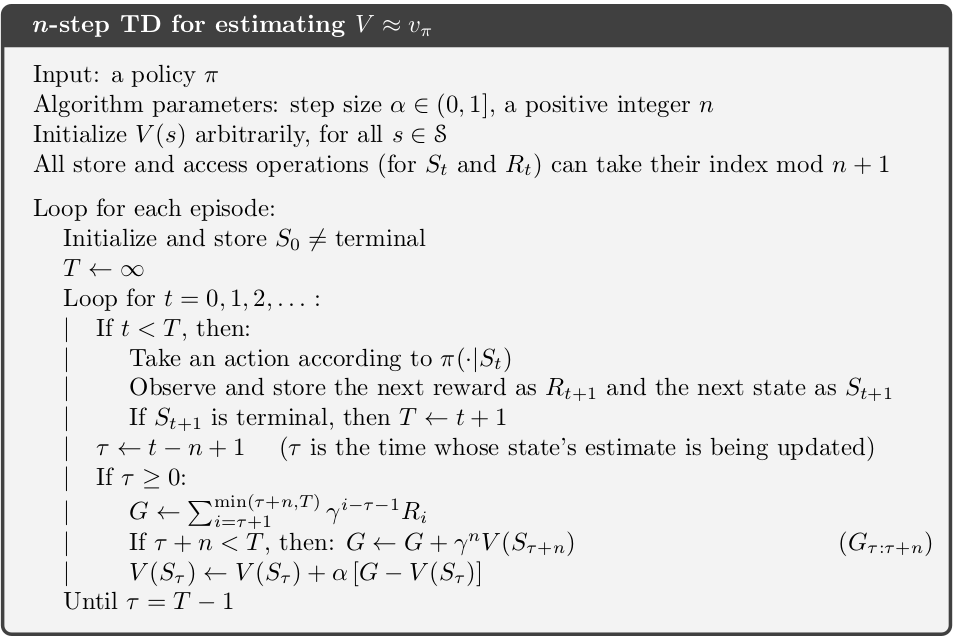
\includegraphics[width=\textwidth]{img/alg_n_step_td.png}
\end{center}

\section{$n$-step Sarsa}
\label{sec:n_step_sarsa}

\begin{myequation}{7.5}
    G_{t:t+n}\doteq\sum_{k=1}^{n}\gamma^{k-1}R_{t+k}+\gamma^nQ_{t+n-1}(S_{t+n},A_{t+n})\\
    Q_{t+n}(S_t,A_t)\doteq
        Q_{t+n-1}(S_t,A_t)+\alpha\left[G_{t:t+n}-Q_{t+n-1}(S_t,A_t)\right]
\end{myequation}

\begin{center}
    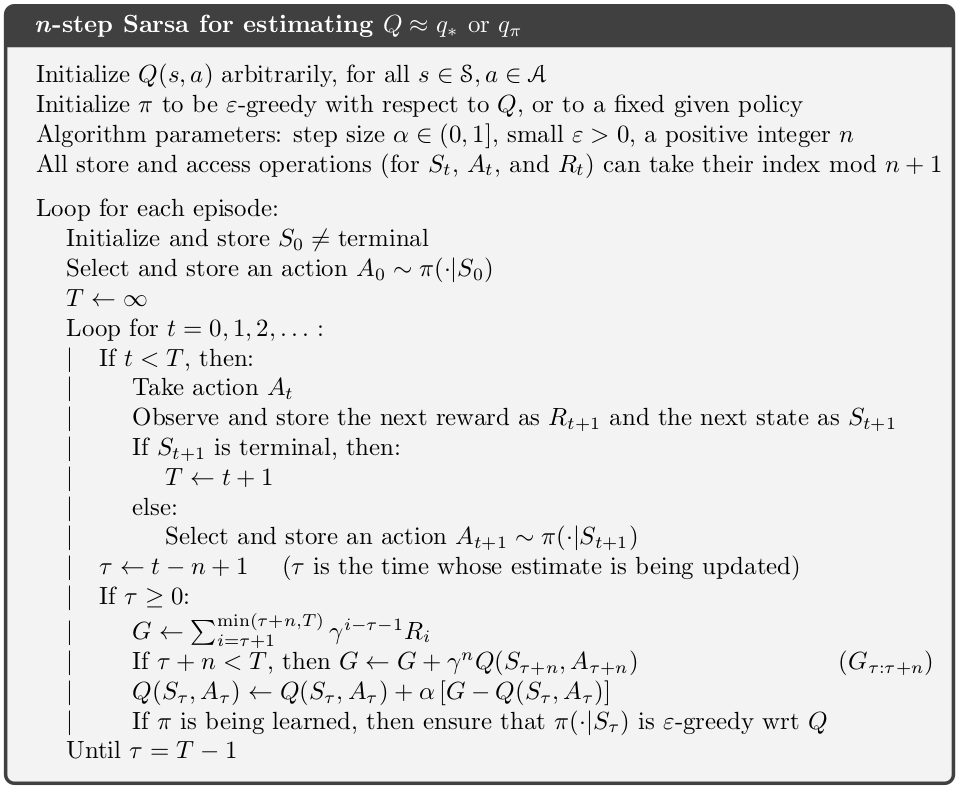
\includegraphics[width=\textwidth]{img/alg_n_step_sarsa.png}
\end{center}

\section{$n$-step Off-policy Learning}
\label{sec:n_step_off_policy_learning}
Other than the $\alpha$, the difference of gain and current value function value is weighted by
$\rho_{t:t+n-1}$.

\begin{myequation}{7.9}
    V_{t+n}(S_t)\doteq V_{t+n-1}(S_t)+\alpha \rho_{t:t+n-1}\left[G_{t:t+n}-V_{t+n-1}(S_t)\right]
\end{myequation}

\begin{myequation}{7.10}
    \rho_{t:h}\doteq\sum_{k=t}^{min(h,T-1)}\frac{\pi(A_k\mid S_k)}{b(A_k\mid S_k)}
\end{myequation}

\begin{myequation}{7.11}
    Q_{t+n}(S_t,A_t)\doteq
        Q_{t+n-1}(S_t,A_t)+\alpha \rho_{t+1:t+n}\left[G_{t:t+n}-Q_{t+n-1}(S_t,A_t)\right]
\end{myequation}

Note that here the \myref{t:importance_sampling_ratio}{importance sampling ratio} ($\rho$)
starts and ends one step later in comparison to the state-value function.
This is because we are not bothered with the current action taken, but rather only
looking at future actions.

\begin{center}
    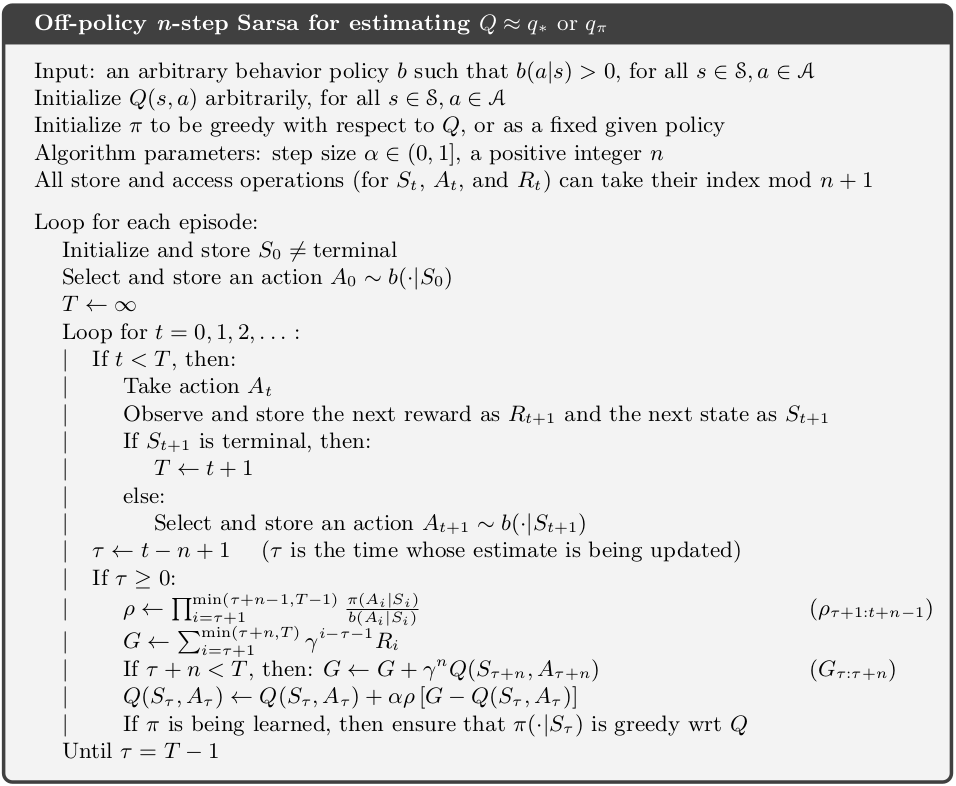
\includegraphics[width=\textwidth]{img/alg_off_policy_n_step_sarsa.png}
\end{center}


\section{*Per-decision Methods with Control Variates}
\label{sec:per_decision_methods_with_control_variates}
This approach takes a similar path to that in section
\ref{sec:per_decision_importance_sampling}.
\begin{myequation}{7.13}
    G_{t:h}\doteq\rho_t(R_{t+1}+\gamma G_{t+1:h})+(1-\rho_t)V_{h-1}(S_t) \\
    \rho_t\doteq \frac{\pi(A_t\mid S_t)}{b(A_t\mid S_t)} \hfill
    G_{h:h}\doteq V_{h-1}(S_h)
\end{myequation}

The $(1-\rho_t)V_{h-1}(S_t)$ term is called the \emph{control variate}\label{t:control_variate}.
It is used to take the value of the resulting state as the approximation of the gain following it.
This term has an effect on $G_{t:h}$ only when $b$ takes actions that are improbable in $pi$.

For a conventional n-step method, the learning rule to use in conjunction with (\ref{eq:7.13})
is the n-step TD update (\ref{eq:7.2}), which has no explicit importance sampling ratios other
than those embedded in the return.

\begin{myequation}{7.14}
    G_{t:h}\doteq
        R_{t+1}+\gamma\rho_{t+1}(G_{t+1:h}-Q_{h-1}(S_{t+1},A_{t+1}))
        +\gamma\bar{V}_{h-1}(S_t+1)\\
        \bar{V}_t(s)\doteq \sum_a\pi(a\mid s)Q_t(s,a) \\
        h<T\Rightarrow G_{h:h}\doteq Q_{h-1}(S_h,A_h)\\
        h\geq T\Rightarrow G_{T-1:h}\doteq R_T
\end{myequation}

\section{Off-policy Learning Without Importance Sampling: The $n$-step Tree Backup Algorithm}
\label{sec:off_policy_learning_without_importance_sampling}

\begin{wrapfigure}[14]{l}{0.2\textwidth}
    \centering
    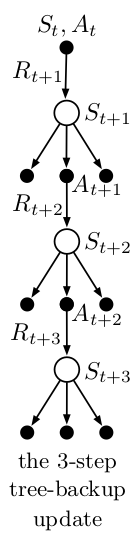
\includegraphics[width=0.2\textwidth]{img/n_step_tree_backup_diagram.png}
\end{wrapfigure}
This algorithm takes into consideration actions not taken.
We go down the taken action to calculate the $G$ but add to it the possibility of taking
and the value of actions \textbf{not taken}.
The last node's gain is calculated just like for \myref{sec:expected_sarsa}{expected sarsa}.
\begin{myequation}{7.15}
    G_{t:t+1}\doteq R_{t+1}+\gamma\sum_{a}\pi(a\mid S_{t+1})Q_t(S_{t+1},a)\\
    \begin{aligned}
        G_{t:t+2}\doteq
        &R_{t+1}+\gamma\sum_{a\neq A_{t+1}}\pi(a\mid S_{t+1})Q_{t+1}(S_{t+1},a)\\
        &+\gamma\pi(A_{t+1}\mid S_{t+1})G_{t+1:t+2}
    \end{aligned}
\end{myequation}
Generalizing to:
\begin{myequation}{7.16}
    \begin{aligned}
        G_{t:t+n}\doteq
        &R_{t+1}+\gamma\sum_{a\neq A_{t+1}}\pi(a\mid S_{t+1})Q_{t+1}(S_{t+1},a)\\
        &+\gamma\pi(A_{t+1}\mid S_{t+1})G_{t+1:t+n}
    \end{aligned} \\
    G_{T-1:t+n}\doteq R_T
\end{myequation}
The update rule is the same as in the $n$-step Sarsa:
\begin{equation*}
    Q_{t+n}\doteq Q_{t+n-1}(S_t,A_t)+\alpha\left[G_{t:t+n}-Q_{t+n-1}(S_t,A_t)\right]
\end{equation*}

\begin{center}
    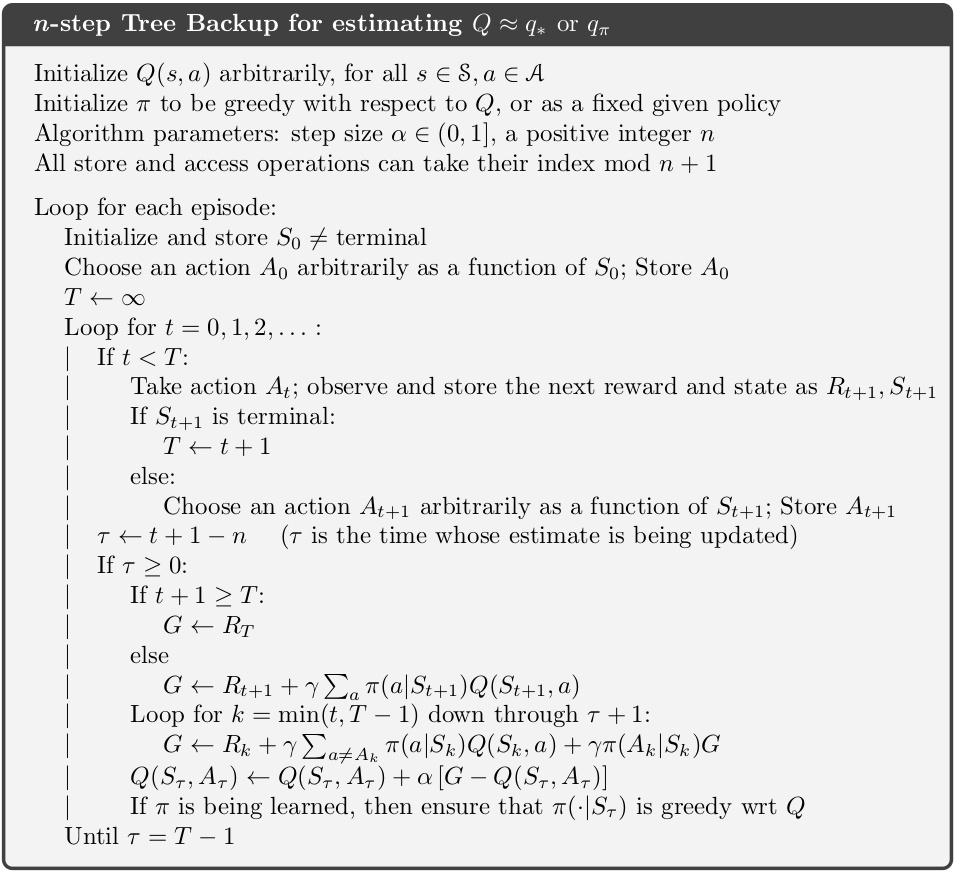
\includegraphics[width=\textwidth]{img/alg_n_step_tree_backup.png}
\end{center}

\section{*A Unifying Algorithm: $n$-step $Q(\sigma)$}
\label{sec:a_unifying_algorithm_n_step_q_sigma}

\begin{center}
    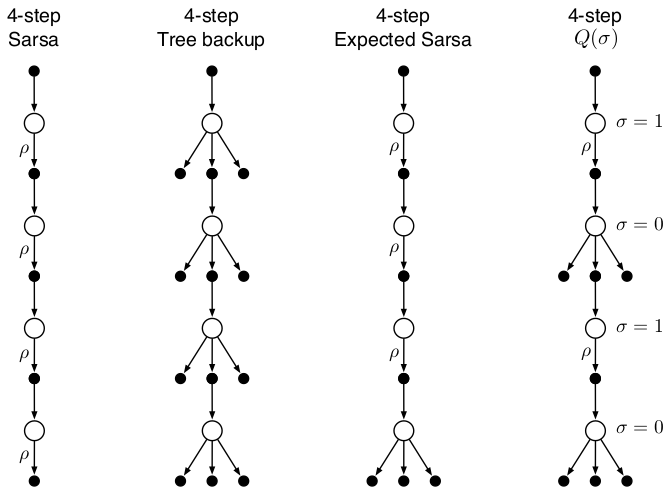
\includegraphics[width=\textwidth]{img/n_step_q_sigma_backup_diagram.png}
\end{center}

Depending on the \emph{random} variable $\sigma\in[0,1]$ the algorithm either samples
with \myref{t:importance_sampling_ratio}{importance sampling} or
calculates via expectations and $\pi$.
$\sigma$ can be a function of $t$, $s$, $(s,a)$,...

\begin{myequation}{7.17}
    \begin{aligned}
        G_{t:h}\doteq
            R_{t+1}+&\gamma\left(
                \sigma_{t+1}\rho_{t+1}
                +(1-\sigma_{t+1})\pi(A_{t+1}\mid S_{t+1})\right)
            \left(G_{t+1:h}-Q_{h-1}(S_{t+1},A_{t+1})\right)\\
            +&\gamma\bar{V}_{h-1}(S_{t+1})
    \end{aligned} \\
    \begin{aligned}
        &G_{h:h}\doteq Q_{h-1}(S_h,A_h), &h<T \\
        &G_{T-1:h}\doteq R_T, &h==T
    \end{aligned}
\end{myequation}
The update rule is the same as in the $n$-step Sarsa:
\begin{equation*}
    Q_{t+n}\doteq Q_{t+n-1}(S_t,A_t)+\alpha\left[G_{t:t+n}-Q_{t+n-1}(S_t,A_t)\right]
\end{equation*}

\begin{center}
    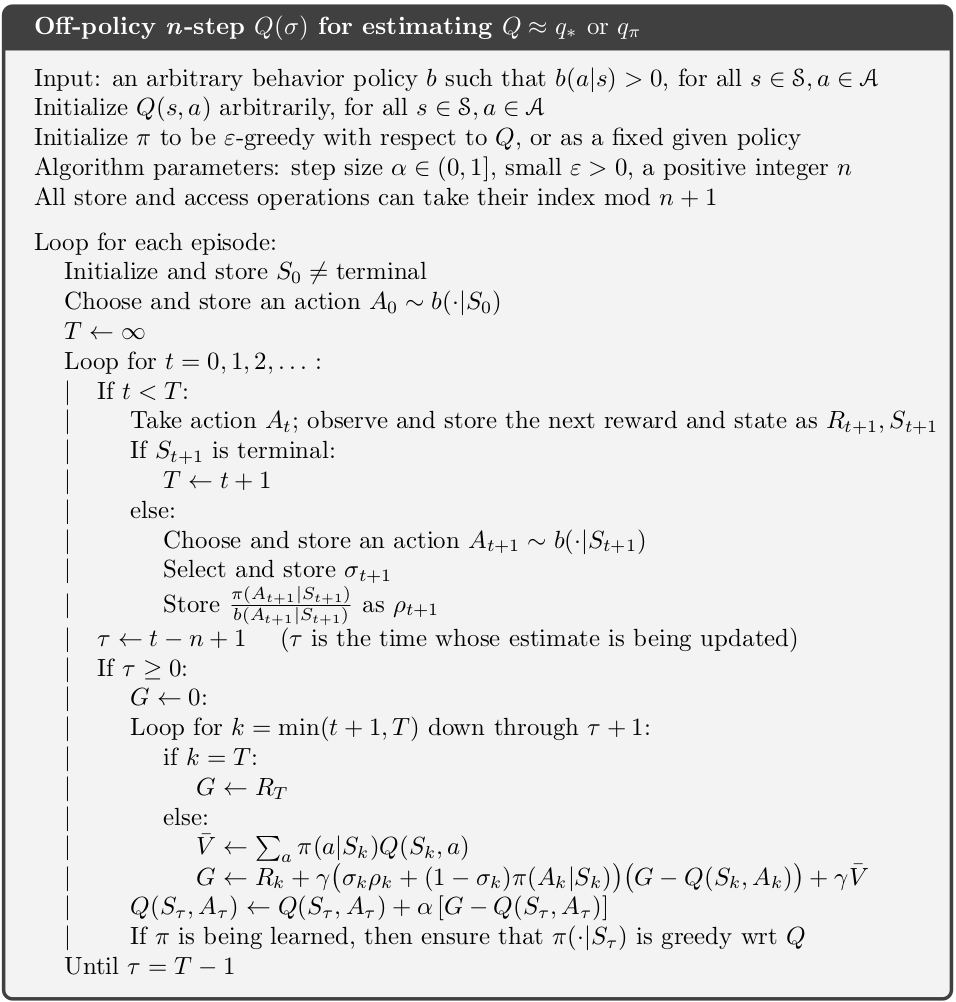
\includegraphics[width=\textwidth]{img/alg_n_step_q_sigma.png}
\end{center}

\section{Summary}
\label{sec:nsb-summary}
In this chapter we have developed a range of temporal-difference learning methods that lie
in between the one-step TD methods of the previous chapter and the Monte Carlo methods
of the chapter before.
Methods that involve an intermediate amount of bootstrapping are important because they will
typically perform better than either extreme.
Our focus in this chapter has been on $n$-step methods, which look ahead to the next $n$ rewards,
states, and actions.
All $n$-step methods involve a delay of $n$ timesteps before updating, as only then are all the
required future events known.
A further drawback is that they involve more computation per timestep than previous methods.
Compared to one-step methods, $n$-step methods also require more memory to record the states,
actions, rewards, and sometimes other variables over the last $n$ time steps.
Eventually, in Chapter 12, we will see how multi-step TD methods can be implemented with
minimal memory and computational complexity using eligibility traces, but there will always be some
additional computation beyond one-step methods.
Such costs can be well worth paying to escape the tyranny of the single time step.
Although $n$-step methods are more complex than those using eligibility traces, they have
the great benefit of being conceptually clear.
We have sought to take advantage of this by developing two approaches to off-policy learning in
the $n$-step case.
One, based on importance sampling is conceptually simple but can be of high variance.
If the target and behavior policies are very different it probably needs some new algorithmic
ideas before it can be efficient and practical.
The other, based on tree-backup updates, is the natural extension of Q-learning to the multi-step
case with stochastic target policies.
It involves no importance sampling but, again if the target and behavior policies are substantially
different, the bootstrapping may span only a few steps even if $n$ is large.
